\begin{center}
    {\LARGE \textbf{2017有机化学}} \\[2ex]
    {\large 时量180分钟 \quad 满分150分}
\end{center}

\vspace{0.5cm}
\noindent\textbf{注意事项:}
\begin{enumerate}[label=\arabic*., parsep=0pt, itemsep=0pt]
    \item 答题前,考生先将自己的姓名、学号、考场号、座位号填写在答题卡上,将条形码准确粘贴在考生信息条形码粘贴区。
    \item 考试结束后,将本试卷与答题纸一并收回。
    \item 回答各个问题时,将答案写在答题纸上,写在本试卷上无效。
\end{enumerate}

\vspace{0.5cm}
\noindent\textbf{一、选择题（15 pts.）}

\begin{enumerate}[label=\arabic*., itemsep=1.5ex]
    \item 不经过活性中间体即能完成的反应是
    \begin{tasks}(2)
        \task 乙炔与HBr的加成反应
        \task 乙烯的[2+2]环加成反应
        \task 丙酮与乙炔钠的加成反应
        \task 苯的Birch还原反应
    \end{tasks}

    \item 下列碳正离子中最不稳定的是
    
    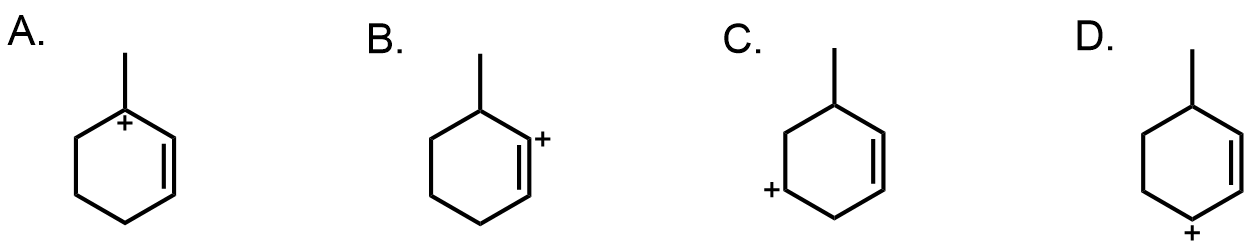
\includegraphics[scale=0.38, valign=c]{./Figure/2017/2017_4_2.png}
    \item 所给出的化合物中不具有芳香性的是
    
    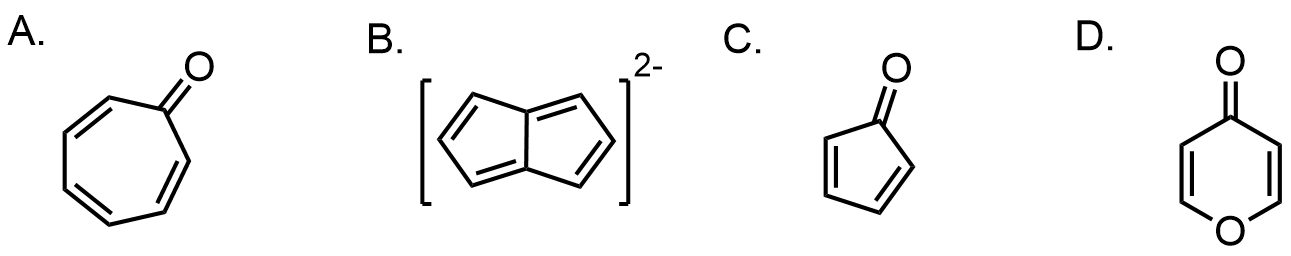
\includegraphics[scale=0.38, valign=c]{./Figure/2017/2017_4_3.png}
    \item (1R,3R)-1-甲基-3-叔丁基环己烷的优势构象是
    
    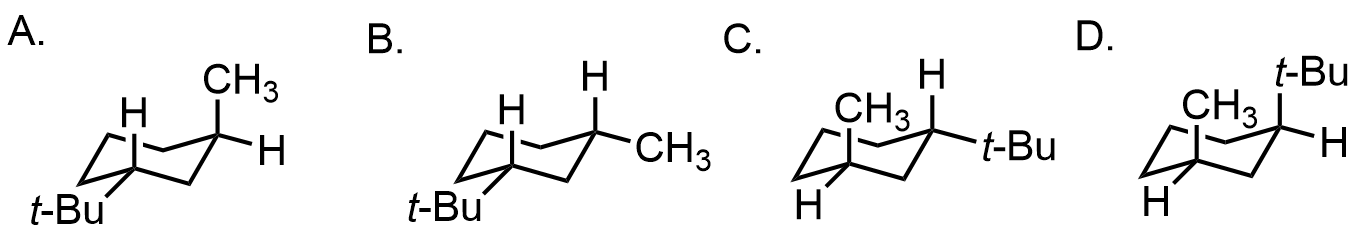
\includegraphics[scale=0.38, valign=c]{./Figure/2017/2017_4_4.png} 
    \item 下列化合物中能与饱和\ce{NaHSO4}水溶液发生反应的是
    
    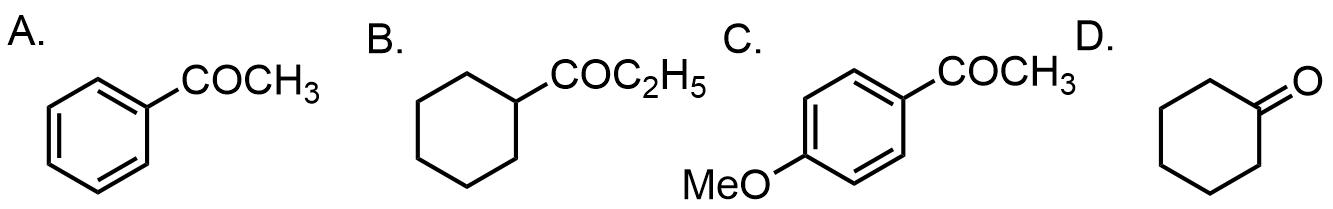
\includegraphics[scale=0.38, valign=c]{./Figure/2017/2017_4_5.png} 
    \item 水蒸气蒸馏结束时，操作顺序如下
    \begin{tasks}(1)
        \task 取下接收瓶，停止加热，旋开水蒸汽发生器与蒸馏瓶之间的螺旋夹
        \task 取下接收瓶，旋开水蒸汽发生器与蒸馏瓶之间的螺旋夹，停止加热
        \task 旋开水蒸汽发生器与蒸馏瓶之间的螺旋夹，停止加热，取下接收瓶
        \task 停止加热，旋开水蒸汽发生器与蒸馏瓶之间的螺旋夹，取下接收瓶
    \end{tasks}
    \item 下列化合物中酸性最大的是
    \begin{tasks}(4)
        \task \ce{CH3COOH}
        \task \ce{CF3CH2COOH}
        \task \ce{CH3CH2COOH}
        \task \ce{CF3COOH}
    \end{tasks}
    \item 满足如下结构的立体异构体数目是

    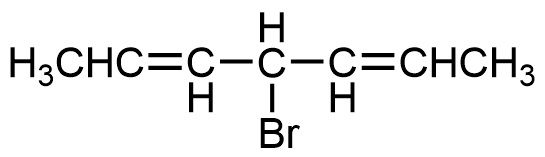
\includegraphics[scale=0.38, valign=c]{./Figure/2017/2017_4_8.png} 
    \begin{tasks}(4)
        \task 2
        \task 4
        \task 6
        \task 8
    \end{tasks}
    \item 预测[16]轮烯中$H_a$的化学位移值(ppm)

    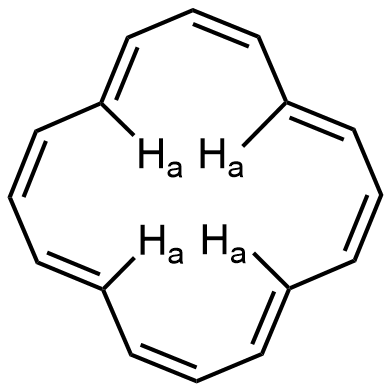
\includegraphics[scale=0.38, valign=c]{./Figure/2017/2017_4_9.png} 
    \begin{tasks}(4)
        \task -3.0
        \task 2.5
        \task 10.6
        \task 1.0
    \end{tasks}
    \item 下列反应中具有立体专一性的是
    \begin{tasks}(1)
        \task 环己烯与\ce{Br2}的加成反应
        \task 1-甲基环丙烷的催化加氢反应
        \task 顺-2-丁烯与三线态卡宾的加成反应
        \task 顺-2-丁烯与单线态卡宾的加成反应
    \end{tasks}
    \item 下列共振式中最稳定的是
    
    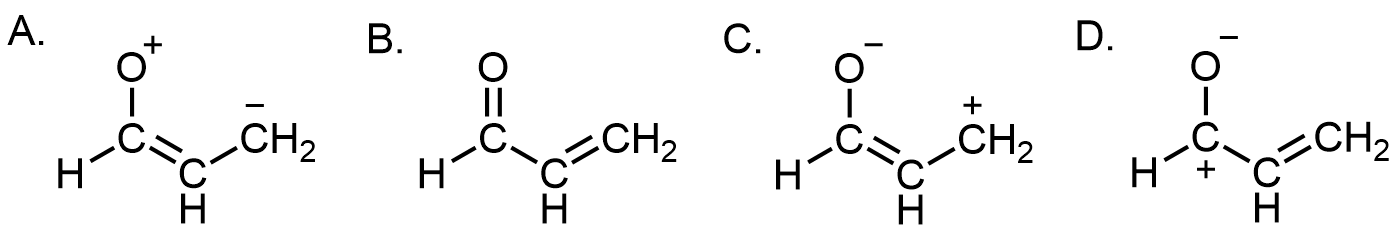
\includegraphics[scale=0.38, valign=c]{./Figure/2017/2017_4_11.png}
    \item 与Lucas试剂反应速度最快的化合物是
    
    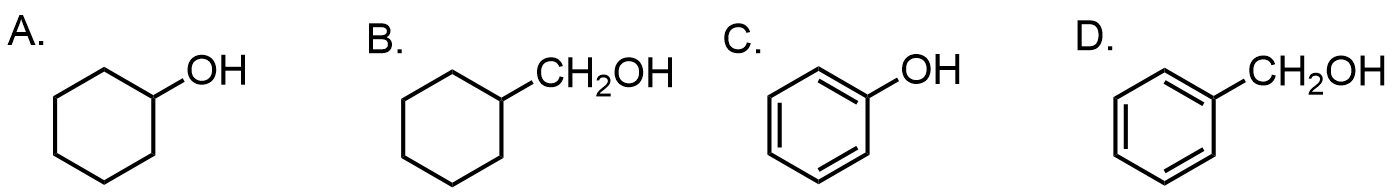
\includegraphics[scale=0.38, valign=c]{./Figure/2017/2017_4_12.png}
    \item 下列叙述正确的是
    \begin{tasks}(1)
        \task 溴苯的磺化反应活性高于吡咯
        \task 溴苯与氨基钠反应的中间体是苯炔
        \task 2,4-二硝基溴苯与氨基钠反应的中间体是苯炔
        \task 苯与\ce{I2}在Fe催化下可制备碘苯
    \end{tasks}
    \item 下列活性中间体的碳原子不是$sp^2$杂化的是
    
    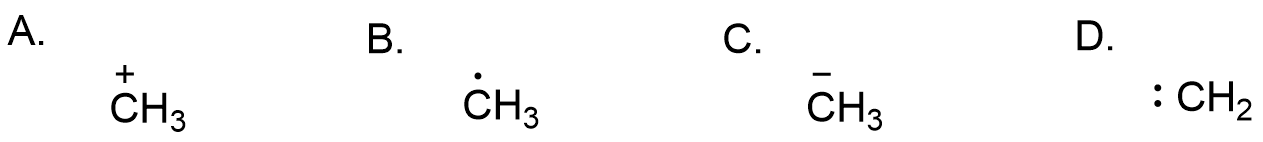
\includegraphics[scale=0.38, valign=c]{./Figure/2017/2017_4_14.png}
    \item 与Lucas试剂反应速度最快的化合物是
    
    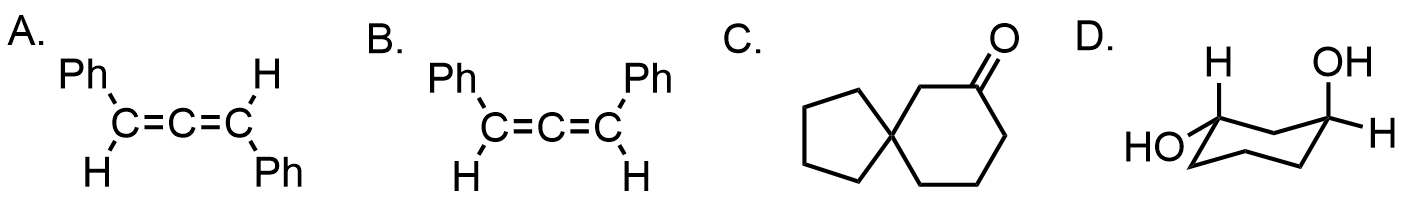
\includegraphics[scale=0.38, valign=c]{./Figure/2017/2017_4_15.png}

\end{enumerate}

\vspace{0.5cm}
\noindent\textbf{二、完成反应(50 pts.)}

\begin{enumerate}[label=\arabic*., itemsep=3ex]
    \item 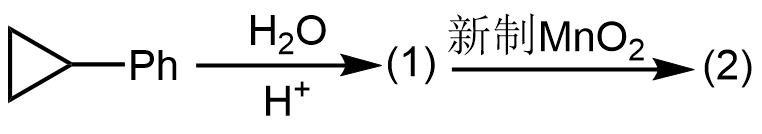
\includegraphics[scale=0.3, valign=c]{./Figure/2017/2017_1_1.png} 
    \item 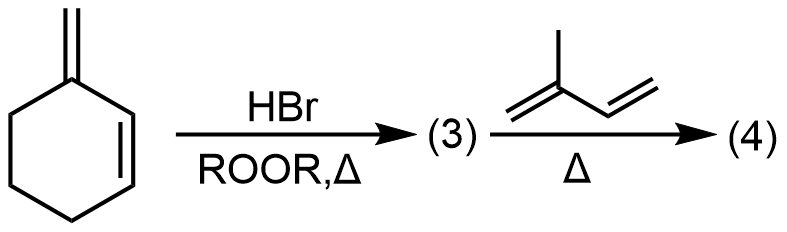
\includegraphics[scale=0.3, valign=c]{./Figure/2017/2017_1_2.png}
    \item 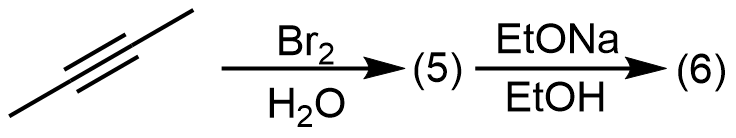
\includegraphics[scale=0.3, valign=c]{./Figure/2017/2017_1_3.png}
    \item 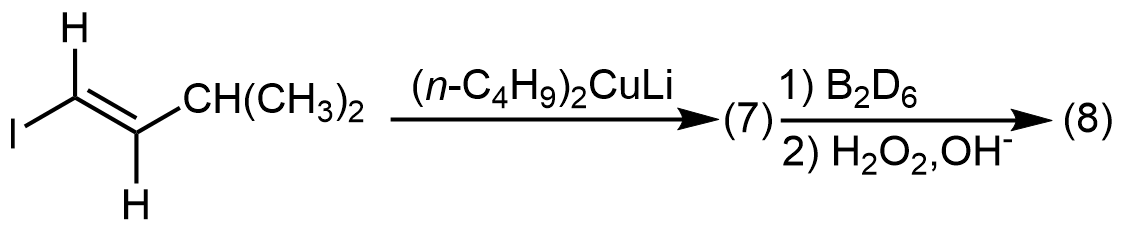
\includegraphics[scale=0.3, valign=c]{./Figure/2017/2017_1_4.png}
    \item 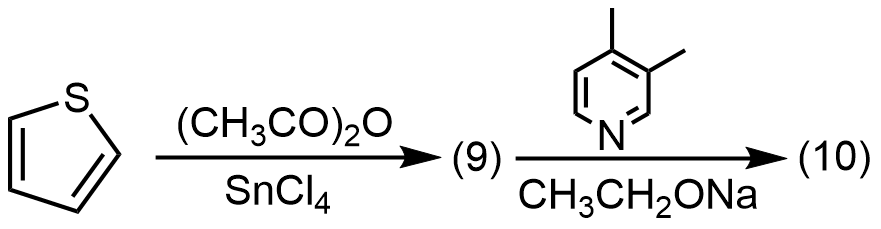
\includegraphics[scale=0.3, valign=c]{./Figure/2017/2017_1_5.png}
    \item 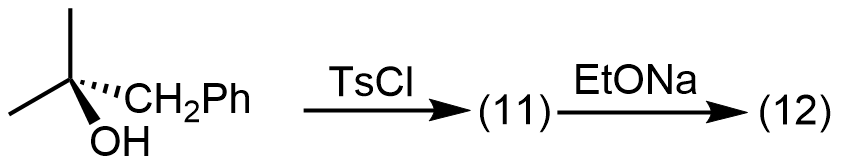
\includegraphics[scale=0.3, valign=c]{./Figure/2017/2017_1_6.png}
    \item 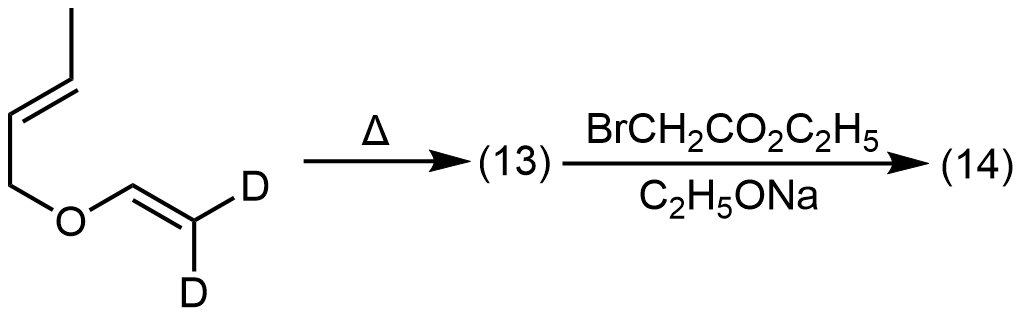
\includegraphics[scale=0.3, valign=c]{./Figure/2017/2017_1_7.png}
    \item 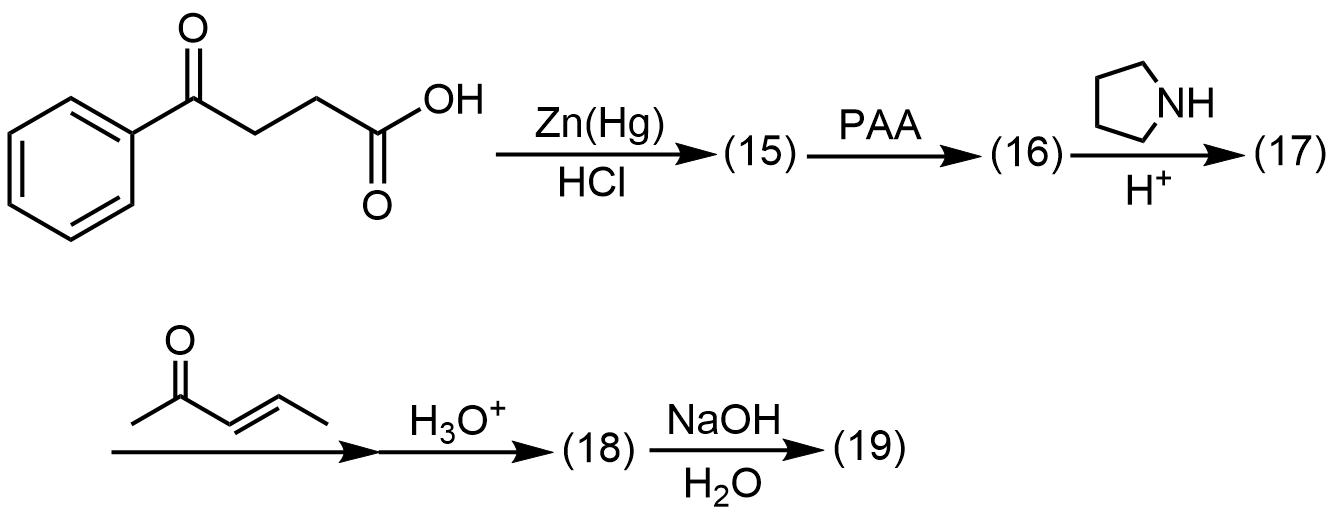
\includegraphics[scale=0.3, valign=c]{./Figure/2017/2017_1_8.png}
    \item 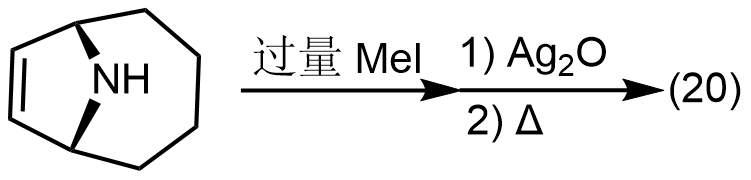
\includegraphics[scale=0.3, valign=c]{./Figure/2017/2017_1_9.png}
    \item 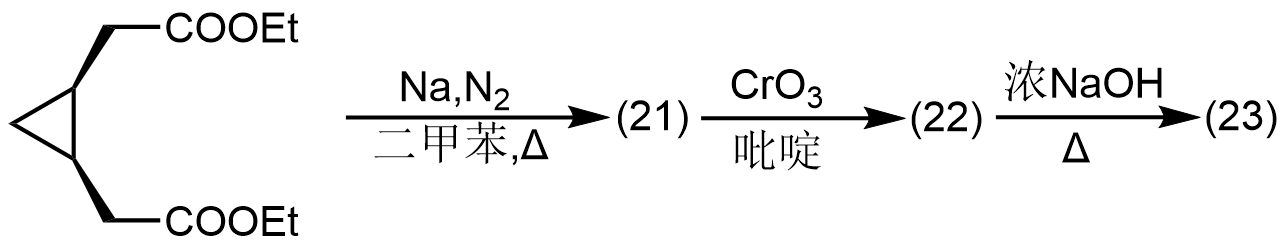
\includegraphics[scale=0.3, valign=c]{./Figure/2017/2017_1_10.png}
    \item 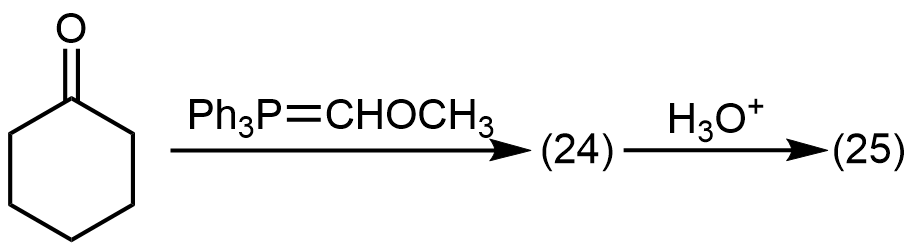
\includegraphics[scale=0.3, valign=c]{./Figure/2017/2017_1_11.png}


\end{enumerate}

\vspace{0.5cm}
\noindent\textbf{三、机理题(28 pts.)}

\begin{enumerate}[label=\arabic*., start=1, itemsep=1.5ex]
    \item 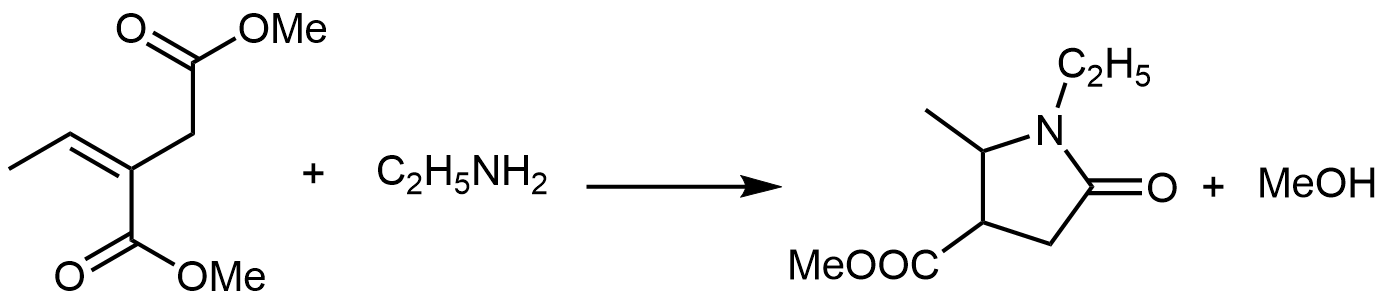
\includegraphics[scale=0.3, valign=c]{./Figure/2017/2017_2_1.png}
    \item 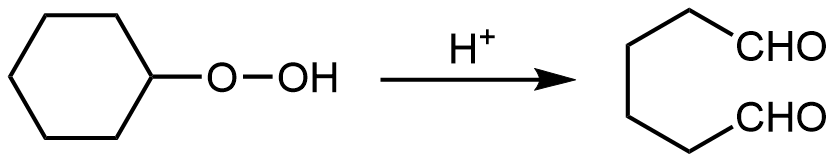
\includegraphics[scale=0.3, valign=c]{./Figure/2017/2017_2_2.png}
    \item 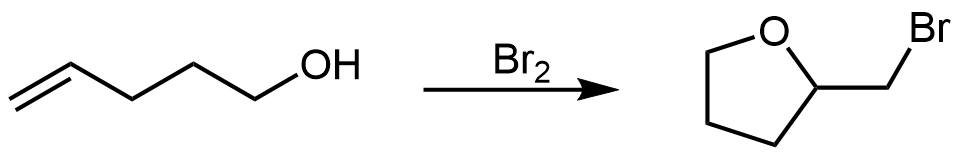
\includegraphics[scale=0.3, valign=c]{./Figure/2017/2017_2_3.png}
    \item 花生四烯酸在铁氧自由基诱导下可被\ce{O2}氧化，生成前列腺素H2的前体，请为如下反应提出合理的机理
    
    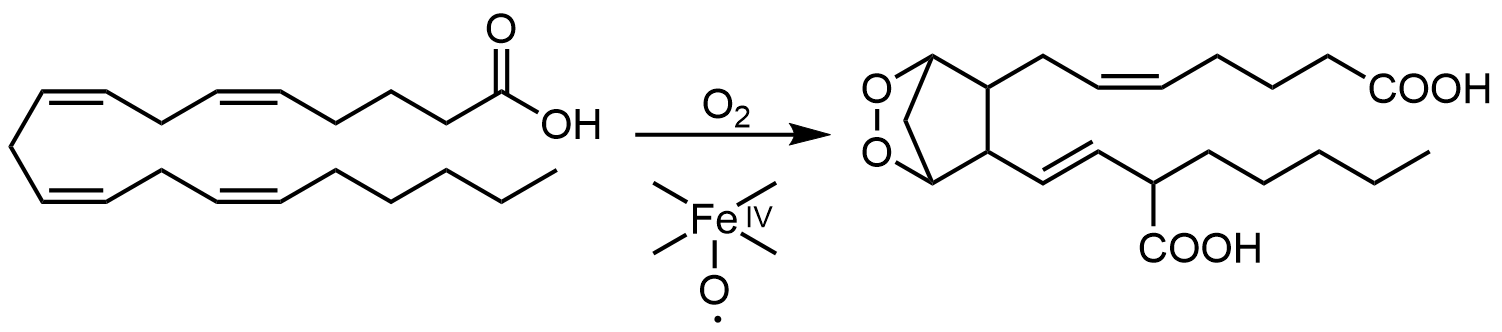
\includegraphics[scale=0.35, valign=c]{./Figure/2017/2017_2_4.png}
\end{enumerate}

\vspace{0.5cm}
\noindent\textbf{四、合成题(42 pts.)}

\begin{enumerate}[label=\arabic*., start=1, itemsep=1.5ex]

    \begin{figure}[htbp]
        \centering
        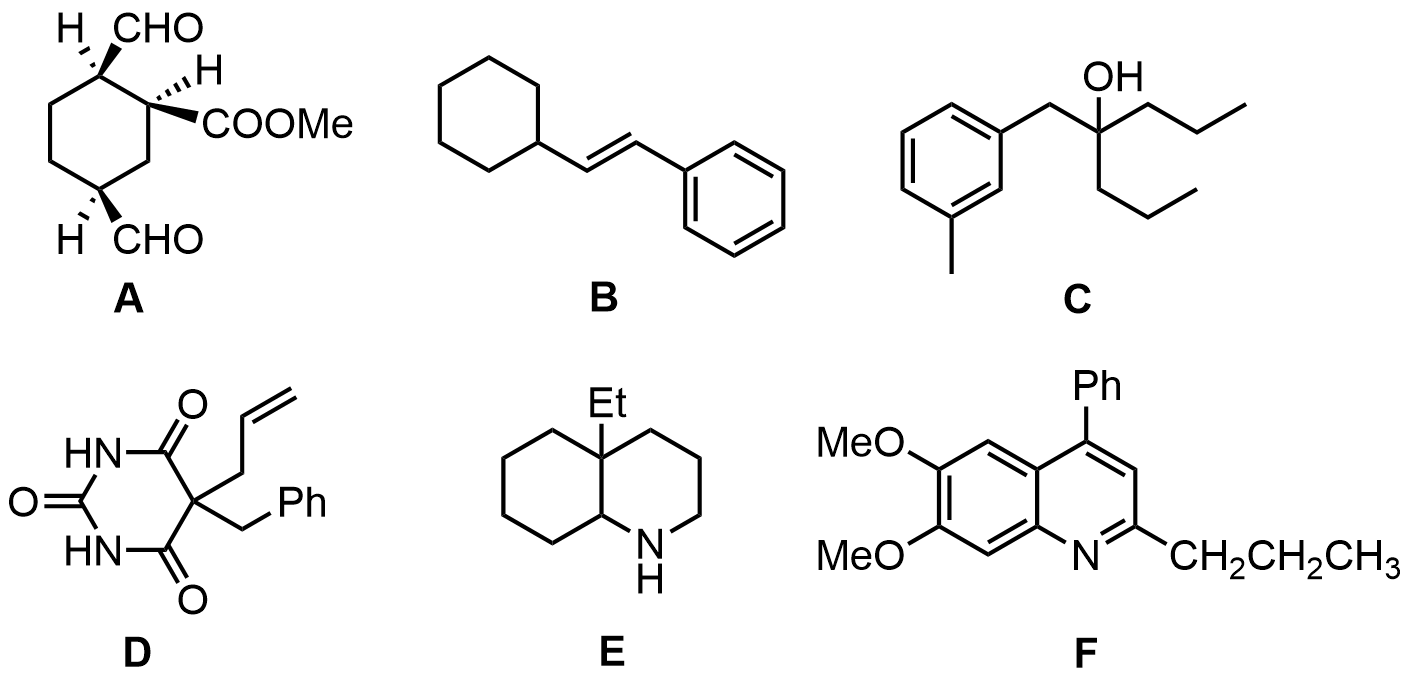
\includegraphics[scale=0.38]{./Figure/2017/2017_3.png}
    \end{figure}
    \item 以乙炔、小于等于3个碳的有机物合成\textbf{A}
    \item 以苯、环己烷、小于等于3个碳的有机物合成\textbf{B}
    \item 以甲苯、小于等于3个碳的有机物合成\textbf{C}
    \item 以丙二酸二乙酯、苯、小于等于3个碳的有机物合成\textbf{D}
    \item 以环己酮、小于等于3个碳的有机物合成\textbf{E}
    \item 以苯、苯甲醚、小于等于4个碳的有机物合成\textbf{F}
\end{enumerate}

\vspace{0.5cm}
\noindent\textbf{五、实验题 略}